\documentclass[tikz,border=7pt]{standalone}
% end preamble
\usepackage[e]{esvect}
\usetikzlibrary{calc, angles}
\tikzset{
  half line/.style = {
    shorten >=-5mm, -latex
  },
  dot/.style = {
    insert path={
      node[scale=2]{.}
    }
  }
}
\begin{document}
  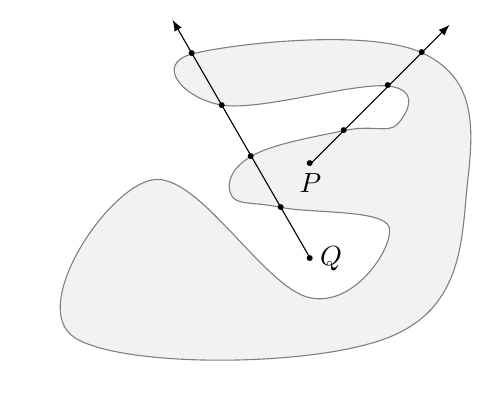
\begin{tikzpicture}
    % les coordonées de P et des Q
    \path
      (0,0) coordinate (Q)
      (120:3) coordinate (Q4)
      ($(Q)!.25!(Q4)$)  coordinate (Q1)
      ($(Q)!.5!(Q4)$)  coordinate (Q2)
      ($(Q)!.75!(Q4)$)  coordinate (Q3)
      (90:1.2) coordinate (P)
      +(45:2) coordinate (P3)
      ($(P)!.3!(P3)$)  coordinate (P1)
      ($(P)!.7!(P3)$)  coordinate (P2)
    ;
    % le domaine
    \path[draw=gray, fill=gray!10, smooth cycle, tension=.7]
      plot coordinates {
        (Q1) (-1,.8) (Q2) (P1) (1.1,1.7) (P2) (Q3) (Q4) (P3)
        (2,1) (1,-1) (-3,-1) (-2,1) (0,-.5) (1,.4)
      }
    ;
    % les rayons
    \path
      (Q) edge[half line] (Q4)
      (P) edge[half line] (P3)
    ;
    % points
    \path
      (Q)  [dot] node[right]{$Q$}
      (Q1) [dot]
      (Q2) [dot]
      (Q3) [dot]
      (Q4) [dot]
      (P)  [dot] node[below]{$P$}
      (P1) [dot]
      (P2) [dot]
      (P3) [dot]
    ;
  \end{tikzpicture}
\end{document}
